\documentclass[10pt,a4paper]{article}
\usepackage[margin=18mm,top=20mm,bottom=19mm,headheight=14pt]{geometry}
\usepackage[T1]{fontenc}
\usepackage{lmodern}
\usepackage{microtype}
\usepackage{xcolor}
\usepackage{tikz}
\usetikzlibrary{arrows.meta,positioning,shapes.geometric}
\usepackage{listings}
\usepackage{tabularx,booktabs,array}
\usepackage{enumitem}
\usepackage{fancyhdr}
\usepackage{titlesec}
\usepackage{hyperref}
\definecolor{ink}{HTML}{142D40}
\definecolor{teal}{HTML}{007F82}
\definecolor{muted}{HTML}{536575}
\definecolor{pale}{HTML}{F0F6F8}
\definecolor{rulegray}{HTML}{D6E1E7}
\definecolor{red}{HTML}{B9424A}
\hypersetup{colorlinks=true,linkcolor=teal,urlcolor=teal}
\renewcommand{\familydefault}{\sfdefault}
\color{ink}
\setlength{\parindent}{0pt}
\setlength{\parskip}{5pt}
\setlength{\emergencystretch}{2em}
\renewcommand{\arraystretch}{1.2}
\setlist[itemize]{leftmargin=16pt,itemsep=2pt,topsep=2pt}
\setlist[enumerate]{leftmargin=18pt,itemsep=2pt,topsep=2pt}
\titleformat{\section}{\Large\bfseries\color{ink}}{\textcolor{teal}{\thesection\enspace}}{0pt}{}
\titleformat{\subsection}{\normalsize\bfseries\color{teal}}{}{0pt}{}
\titlespacing*{\section}{0pt}{9pt}{7pt}
\titlespacing*{\subsection}{0pt}{7pt}{3pt}
\pagestyle{fancy}
\fancyhf{}
\fancyhead[L]{\small\textcolor{muted}{NESTJS TP1}}
\fancyhead[R]{\small\textcolor{muted}{Study documentation}}
\fancyfoot[L]{\footnotesize\textcolor{muted}{Explain the responsibility, then the code.}}
\fancyfoot[R]{\small\thepage}
\renewcommand{\headrulewidth}{0.4pt}
\lstdefinelanguage{TypeScript}{keywords={import,from,export,class,const,let,return,new,private,readonly,constructor,async,await,if,throw,extends,string,number,boolean,void,true,false,enum},sensitive=true,comment=[l]{//},morecomment=[s]{/*}{*/},morestring=[b]',morestring=[b]"}
\lstset{language=TypeScript,basicstyle=\ttfamily\footnotesize,keywordstyle=\color{teal}\bfseries,commentstyle=\color{muted},stringstyle=\color{red},backgroundcolor=\color{pale},frame=single,rulecolor=\color{rulegray},framerule=0.4pt,framesep=6pt,xleftmargin=6pt,xrightmargin=6pt,breaklines=true,columns=fullflexible,keepspaces=true,showstringspaces=false,tabsize=2,aboveskip=7pt,belowskip=6pt}
\newcommand{\code}[1]{\texttt{#1}}
\newcommand{\note}[1]{\par\smallskip\noindent\colorbox{pale}{\parbox{\dimexpr\linewidth-12pt}{\vspace{4pt}\textcolor{teal}{\textbf{Remember}} \ #1\vspace{4pt}}}\par\smallskip}
\tikzset{box/.style={draw=rulegray,fill=pale,rounded corners=3pt,align=center,minimum height=11mm,text width=38mm,font=\small},accent/.style={box,draw=teal,fill=teal!7},arr/.style={-{Latex[length=2mm]},thick,draw=teal}}
\begin{document}


\hypersetup{pdftitle={TP1 NestJS Defense Guide},pdfauthor={Yassine}}
\thispagestyle{empty}
{\small\bfseries\color{teal} NESTJS / RT4 TP1 / PROFESSOR-FACING NOTES}\par\vspace{10mm}
{\fontsize{31}{35}\selectfont\bfseries TP1 Defense Guide\par}\vspace{4mm}
{\Large What I built, why I built it, and how to explain it\par}
\vspace{5mm}{\color{muted} Completed through slide 5 / TypeORM connection}\par\vspace{8mm}
This document describes the actual state of the project at handoff. It is designed for a technical explanation: every file has a role, every decorator has a reason, and the next unfinished exercise is clearly identified.
\begin{center}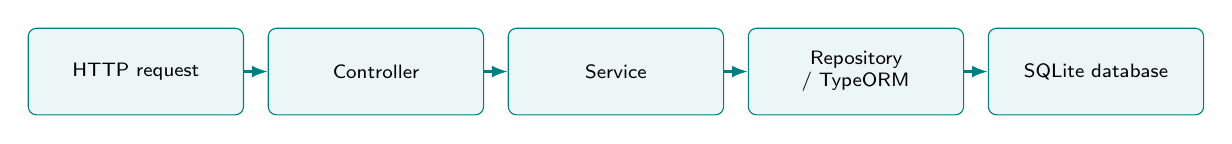
\begin{tikzpicture}[node distance=3mm]
\node[accent,text width=25mm,font=\scriptsize] (a) {HTTP request};
\node[accent,text width=25mm,font=\scriptsize,right=of a] (b) {Controller};
\node[accent,text width=25mm,font=\scriptsize,right=of b] (c) {Service};
\node[accent,text width=25mm,font=\scriptsize,right=of c] (d) {Repository / TypeORM};
\node[accent,text width=25mm,font=\scriptsize,right=of d] (e) {SQLite database};
\draw[arr](a)--(b);\draw[arr](b)--(c);\draw[arr](c)--(d);\draw[arr](d)--(e);
\end{tikzpicture}\end{center}
\note{The implementation currently demonstrates Nest modules, a custom value provider, constructor injection, one test endpoint, a TypeORM entity, and a working SQLite connection. Todo validation and CRUD are still future work.}
\begin{tabularx}{\linewidth}{@{}lX@{}}\toprule
\textbf{Project} & \code{todo-api}\\
\textbf{Location} & \code{/home/yassine/Desktop/TP1-NestJS/todo-api}\\
\textbf{Framework} & NestJS 11 with TypeScript\\
\textbf{Database} & SQLite through the supported \code{better-sqlite3} driver\\
\textbf{Current endpoint} & \code{GET /uuid-test} returns a newly generated UUID\\\bottomrule
\end{tabularx}
\vfill\textcolor{muted}{Generated from the working project on 19 October 2026.}

\newpage
\section{The professor's expected reasoning}
The TP1 instructions emphasize four habits. They are course requirements, not code features:
\begin{itemize}
\item Understand every line well enough to explain it without reading it for the first time during the interview.
\item Think about architecture before adding code.
\item Keep code coherent, readable, reusable, and properly divided into modules.
\item Treat validation like a technical interview: explain decisions, tradeoffs, and failure cases.
\end{itemize}
When explaining this project, start with responsibility rather than syntax:
\begin{tabularx}{\linewidth}{@{}lX@{}}\toprule
\textbf{Piece} & \textbf{Responsibility}\\\midrule
Module & Organizes controllers and providers and controls what is shared.\\
Controller & Receives HTTP requests and returns responses.\\
Service & Contains application behavior.\\
Provider & Gives Nest a dependency under a token.\\
Entity & Maps a class to a database table.\\
TypeORM & Connects the entity to a database.\\\bottomrule
\end{tabularx}

\section{Project creation}
The project was generated with the Nest CLI using a version compatible with the installed Node.js version. The generated application starts at \code{src/main.ts} and bootstraps \code{AppModule}.
\begin{lstlisting}
async function bootstrap() {
  const app = await NestFactory.create(AppModule);
  await app.listen(process.env.PORT ?? 3000);
}
bootstrap();
\end{lstlisting}
\code{NestFactory.create(AppModule)} builds Nest's dependency graph. \code{listen(...)} starts the HTTP server. The root module is the assembly point; requests do not execute through the module class as an extra layer.
The original generated route is in \code{src/app.controller.ts}. Its controller calls \code{AppService.getHello()}, which returns \code{Hello World!}. This proved that the application starts and routes requests correctly.

\section{CommonModule and UUID provider}
\subsection{Why a common module?}
The assignment asks for a module that will be used frequently. The project therefore has \code{src/common/common.module.ts}. It is marked global because it exposes a reusable dependency across the application.
\begin{lstlisting}
@Global()
@Module({
  providers: [
    {
      provide: UUID_PROVIDER,
      useValue: uuidv4,
    },
  ],
  exports: [UUID_PROVIDER],
})
export class CommonModule {}
\end{lstlisting}
\subsection{Why useValue?}
The UUID library exports an existing function. Nest does not need to instantiate a class or calculate a one-time value. \code{useValue: uuidv4} places the function itself in the dependency-injection container. Each consumer can call it and obtain a new UUID.
The project deliberately avoids \code{useValue: uuidv4()}. That would execute the generator once during startup and inject one fixed string. It also does not use \code{useClass}, because \code{uuidv4} is a function, not a class.
The provider token is a symbol in \code{src/common/constants/common.constants.ts}:
\begin{lstlisting}
export const UUID_PROVIDER = Symbol('UUID_PROVIDER');
\end{lstlisting}
The symbol is the runtime key. Since it is not a class, consumers must use \code{@Inject(UUID\_PROVIDER)} explicitly.

\section{Dependency-injection proof}
The test feature is under \code{src/uuid-test/}. It has a module, service, and controller. The service receives the UUID function through its constructor:
\begin{lstlisting}
@Injectable()
export class UuidTestService {
  constructor(
    @Inject(UUID_PROVIDER)
    private readonly generateUuid: () => string,
  ) {}

  generate() {
    return { id: this.generateUuid() };
  }
}
\end{lstlisting}
The controller exposes the service through \code{GET /uuid-test}:
\begin{lstlisting}
@Controller('uuid-test')
export class UuidTestController {
  constructor(private readonly uuidTestService: UuidTestService) {}

  @Get()
  generate() {
    return this.uuidTestService.generate();
  }
}
\end{lstlisting}
Refreshing the endpoint produces a different UUID because the injected value is a generator function and the service calls it for every request.
\begin{center}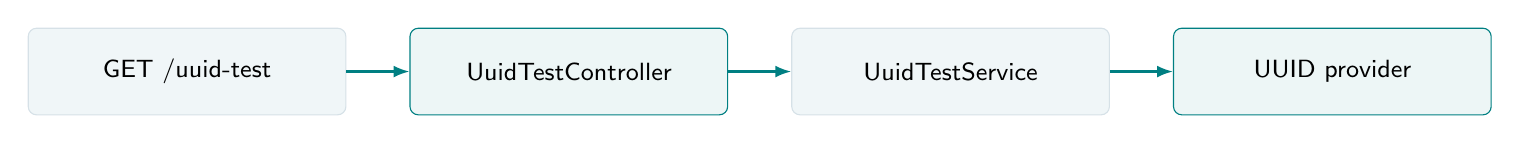
\begin{tikzpicture}[node distance=8mm]
\node[box] (r) {GET /uuid-test};
\node[accent,right=of r] (c) {UuidTestController};
\node[box,right=of c] (s) {UuidTestService};
\node[accent,right=of s] (u) {UUID provider};
\draw[arr](r)--(c);\draw[arr](c)--(s);\draw[arr](s)--(u);
\end{tikzpicture}\end{center}

\section{TodoEntity}
The first database model is in \code{src/todos/entities/todo.entity.ts}. Its enum is in \code{src/todos/enums/status.enum.ts}. The assignment says the status enum was already defined in an earlier exercise; this project uses the temporary values \code{TODO}, \code{IN\_PROGRESS}, and \code{DONE} until the course's exact enum is confirmed.
\begin{lstlisting}
@Entity('todos')
export class TodoEntity {
  @PrimaryGeneratedColumn()
  id!: number;

  @Column()
  name!: string;

  @Column()
  description!: string;

  @CreateDateColumn()
  createdAt!: Date;

  @Column({ type: 'varchar', default: StatusEnum.TODO })
  status!: StatusEnum;
}
\end{lstlisting}
\begin{tabularx}{\linewidth}{@{}lX@{}}\toprule
\textbf{Decorator} & \textbf{Meaning}\\\midrule
\code{@Entity('todos')} & Maps the class to the \code{todos} table.\\
\code{@PrimaryGeneratedColumn()} & Integer primary key generated by the database.\\
\code{@Column()} & Ordinary persisted column.\\
\code{@CreateDateColumn()} & Creation time managed by TypeORM.\\\bottomrule
\end{tabularx}
An entity describes stored data. A later DTO will describe data allowed from an HTTP client. Generated fields such as \code{id} and \code{createdAt} must not be accepted as ordinary client input.

\section{TypeORM configuration}
The TypeORM setup is in \code{src/app.module.ts}:
\begin{lstlisting}
TypeOrmModule.forRoot({
  type: 'better-sqlite3',
  database: 'todo.sqlite',
  entities: [TodoEntity],
  synchronize: true,
}),
\end{lstlisting}
\code{forRoot(...)} creates the application-level connection and tells TypeORM which entities to map. The local database is the file \code{todo.sqlite}. \code{synchronize: true} is suitable for this learning project, but it must not be used in production because automatic schema changes can lose data.
The initial attempt used \code{type: 'sqlite'}, but the installed TypeORM version's type definitions support \code{better-sqlite3} instead. The driver was installed and the configuration was changed accordingly. The database file is now created successfully when the application starts.
\note{The future feature module will add \code{TypeOrmModule.forFeature([TodoEntity])}. That registers the Todo repository in the feature module so the service can inject it.}

\section{Verification and current limitations}
Successful checks:
\begin{itemize}
\item \code{npm run build} passes.
\item \code{todo.sqlite} is created.
\item \code{GET /uuid-test} returns a UUID.
\item Repeating the request returns a different UUID.
\end{itemize}
The generated unit tests for \code{UuidTestService} and \code{UuidTestController} currently fail because their isolated testing modules do not register the UUID token and service dependencies. The runtime application is working; these tests need mock providers or imported modules before the test suite can pass.

\section{What remains in TP1}
The next unfinished point is slide 6. The remaining work should be implemented in this order:
\begin{enumerate}
\item Add \code{CreateTodoDto}, validation decorators, centralized messages, and the global \code{ValidationPipe}.
\item Add an optional-field update DTO and validate the status enum.
\item Add \code{updatedAt} and \code{deletedAt}; keep \code{createdAt} outside update input.
\item Extract creation, update, and deletion timestamp columns into a reusable base entity.
\item Create \code{TodosModule}, \code{TodosService}, and \code{TodosController}; register the Todo repository with \code{forFeature}.
\item Implement create, update, hard delete, soft delete, restore, status counts, get-all, get-by-id, filtering, and pagination.
\end{enumerate}

\section{Short answers for an oral explanation}
\begin{tabularx}{\linewidth}{@{}p{55mm}X@{}}\toprule
\textbf{Question} & \textbf{Answer}\\\midrule
Why is UUID a value provider? & The library gives us an existing function; Nest should inject that function.\\
Why is \code{@Inject} needed? & The token is a symbol, so Nest cannot infer it from a class type.\\
Why export the token? & A provider must be exported to be available outside its declaring module.\\
Why global CommonModule? & It is intended for frequent shared use, so importing it everywhere is unnecessary.\\
What does the entity do? & It maps the Todo class and its decorators to the database table structure.\\
What does \code{forRoot} do? & It configures the application's TypeORM connection.\\
What does \code{synchronize} do? & It synchronizes the development schema from entity metadata.\\
Why is the DTO separate? & Input rules and persisted database structure are different responsibilities.\\\bottomrule
\end{tabularx}

\subsection*{Useful commands}
\begin{lstlisting}[language={}]
npm run build
npm run format
npm run start:dev
curl http://localhost:3000/uuid-test
\end{lstlisting}
\end{document}
